\documentclass[11pt,a5paper]{article}
\usepackage[utf8]{inputenc}
\usepackage{german}
\usepackage{amsmath}
\usepackage{amsfonts}
\usepackage{amssymb}
\usepackage{textcomp}
\usepackage[width=11.80cm, height=18.00cm]{geometry} % 1,5 cm auf allen vier Seiten
\usepackage{tabularx}
\usepackage{graphics}
\usepackage{graphicx}
\usepackage{wrapfig}
\usepackage{mathtools}
\usepackage[percent]{overpic}
\usepackage[absolute]{textpos}
\usepackage{beramono}
\usepackage{ascii}
\usepackage[T1]{fontenc}
\usepackage{titlesec}
\usepackage[most]{tcolorbox}
\usepackage{color}

% Clickable ToC, see http://tex.stackexchange.com/a/73865
\usepackage{hyperref}
\hypersetup{
	colorlinks,
	citecolor=black,
	filecolor=black,
	linkcolor=black,
	urlcolor=black
}

% Farbgebung
\newcommand\chordcolor{blue}
\newcommand\refboxcolor{gray!17}
\newcommand\colorjoke{red}

% Kästen um Refrains herum
\tcbset{
	frame code={}
	center title,
	left=0pt,
	right=0pt,
	top=0pt,
	bottom=0pt,
	colback=\refboxcolor,
	colframe=white,
	width=\dimexpr\textwidth\relax,
	enlarge left by=0mm,
	boxsep=5pt,
	arc=0pt,outer arc=0pt,
}

%\titleformat{\section}[display]{\normalfont\asciifamily\Large\bfseries}{\chaptertitlename\ \thechapter}{15pt}{\Large}
%\titleformat{\subsection}[display]{\normalfont\asciifamily\large\bfseries}{\chaptertitlename\ \thechapter}{15pt}{\large}

%\renewcommand{\familydefault}{\asciifamily}

% Keine Nummerierung von (Unter-)Kapiteln
\setcounter{secnumdepth}{-1}

\setlength{\TPHorizModule}{\paperwidth}\setlength{\TPVertModule}{\paperheight}
\renewcommand{\familydefault}{\sfdefault}
\setlength{\parindent}{0cm}

% Setzen von Akkorden
\newcommand\chord[2][l]{\makebox[0pt][#1]{\begin{tabular}[b]{@{}l@{}}\textcolor{\chordcolor}{#2}\\\mbox{}\end{tabular}}}

% Refrain-Hervorhebung und -Referenzierung
\newcommand\refrain[1]{\begin{tcolorbox}#1\end{tcolorbox} \ }
\newcommand{\refrefrain}{\refrain{\textsc{Refrain}} \ }
\newcommand{\refrefraintwice}{\refrain{\textsc{2x Refrain}} \ }
\newcommand{\refrefrainthreetimes}{\refrain{\textsc{3x Refrain}} \ }

% Infos zum Lied im oberen rechten Eck
\newcommand\songinfo[2]{\begin{textblock}{0.5}(0.41,0.065)
		\footnotesize 
		\hfill \textit{Original:} \ \ \ \ \ \ \ \ \ \ \ \ \ \ \ \ \ \ \ \ 
		
		\hfill #1
		
		\hfill  \textit{Text:} \ \ \ \ \ \ \ \ \ \ \ \ \ \ \ \ \ \ \ \ 
		
		\hfill #2
	\end{textblock}}
	
% Kürzere Infos, nur über zwei Zeilen (Fix, damit Infos nicht in Refrain-Kasten ragen)
\newcommand\songinfoshort[2]{\begin{textblock}{0.5}(0.41,0.065)
		\footnotesize 
		\hfill \textit{Original:} #1
		
		\hfill  \textit{Text:} #2
	\end{textblock}}
	
% Witz
\newcommand\joke[1]{\textcolor{\colorjoke}{\textsc{#1}}}

% Titelblatt
\def\maketitle{
	\vspace*{0.5cm}
	%\begin{center}
		\begin{overpic}[width=12.5cm]{hacker-cover.pdf}
		\end{overpic}
		%{\Large Wiederverwendbare Liedermodule \\ }
		%\vspace{1cm}
		%{Fachschaft Informatik \& Softwaretechnik, Universität Stuttgart}
	%\end{center}
	}
	
%\makeatother
	
\begin{document}
		
%\title{Wiederverwendbare Liedermodule}
\maketitle
\thispagestyle{empty}
\pagebreak
\tableofcontents
\pagebreak

% Schriftgröße des Dokuments!
\small

\section*{Vorwort}

Liebe Leserin, lieber Leser! \\
			
Fertig kompiliert, Beta-getestet und integriert liegt es nun in deinen Händen, das neue Liederbuch für Informatiker, Softwaretechniker, IT-ler und alle Interessierten. 
Es erwartet dich eine bunte Mischung von zweiundzwanzig selbst-gedichteten Songtexten, die die \glqq Welt der Informatik\grqq \ thematisieren, aber nicht allzu ernst nehmen. Das Digitale nimmt heute so viel Einfluss auf unsere Leben wie noch nie zuvor -- da ist es doch völlig angebracht, auch einmal unsere Smartphones und Computer, und unsere Erlebnisse mit ihnen, ausgiebig zu besingen.

%Auf den nächsten Seiten findest du Lobeshymnen auf \emph{Stack Overflow} und \emph{Python}, Klagelieder über \texttt{git} und \TeX, Liebesbekundungen an die eigene Firewall und den nächsten Wunsch-PC, und vieles mehr. 
Entstanden ist das ganze aus dem Wunsch heraus, den damals von der Stuttgarter Informatik-- und Softwaretechnik-Fachschaft herausgegebenen und mittlerweile etwas in die Jahre gekommenen Liederbüchern \emph{Chor Dump} und \emph{Chor Dump 2} einen würdigen Nachfolger zu bescheren.
Da wir mit der Zeit gehen möchten, heißt der Untertitel des Buches nun natürlich nicht mehr \emph{Effiziente Algorythmen}, sondern \emph{Wiederverwendbare Liedermodule}.

Danken möchten wir Jun.-Prof. Dirk Pflüger, der eines Abends auf der Ferienakademie im schönen Sarntal den Anstoß für die Idee gegeben hat; den fleißigen Fachschaftlern, die tollerweise das Drucken übernommen haben; sowie natürlich allen, die kreative Ideen und Texte für die Lieder eingebracht haben. \\

Damit wäre alles geklärt -- ganz viel Spaß beim Singen! \\

\hfill Dominik Schreiber \\

\ \\

\subsection*{Hinweise}

Die Lieder sind soweit möglich thematisch sortiert; Freunde der Softwareentwicklung beginnen am besten ganz am Anfang, während die \glqq Endbenutzer\grqq \ des Liederbuchs insbesondere auf den Seiten 14 bis 27 auf ihre Kosten kommen. Hymnen auf einzelne, bekannte Institutionen aus der IT-Welt (etwa Linux oder Python) folgen ab Seite 28. Abgerundet wird das Buch durch zwei \glqq Bonus-Lieder\grqq \ spezifisch für die Informatik an der Uni Stuttgart.

\emph{Refrains} sind hinterlegt.
Zu \emph{Strophen} und \emph{Bridges} sind die Akkordfolgen in der Regel einmal angegeben, und werden dann implizit wiederholt. Die Lieder sollte man im Ohr haben, da keine Noten abgedruckt sind.

Die Tonart einiger Lieder wurde zugunsten der Spielbarkeit angepasst.

\pagebreak

\subsection{Branching Tree}
\songinfo{Fool's Garden -- Lemon Tree}{Dominik Schreiber}

I'm \chord{a}sitting here in a \chord{e}boring room \\
The \chord{a}program must compile until to\chord{e}morrow noon \\
I'm \chord{a}wasting my time, looking \chord{e}for a bug \\
For \chord{a}hours and hours I am \chord{e}trying my luck \\
But no\chord{d}thing ever happens \chord{e}- and I wo\chord{a}nder. \chord{e \ \ a} \\

My partner tells me, \glqq Everything's fine, \\
I fixed that problem on my branch for quite some time \\
Just fetch and merge, stage and commit \\
and don't forget to push -- that should be it\grqq \\
But nothing ever happens -- and I wonder. \\

\refrain{
	I \chord{C}wonder how, I \chord{G}wonder why, \chord{a}Git does seem so easy for that \chord{e}other guy \\
	but all\chord{d} that I can see\chord{G} is just the giant \chord{C}branching tree. \chord{G} \\
	I \chord{C}pull and push \chord{G}every time, still \chord{a}merging conflicts haunt me every \chord{e}second line \\
	and all\chord{d} that I can \chord{D}see is just that giant \chord{G}branching tree.}

Sing, \chord{a}Git  \\
\chord{e} Gididi di \chord{a}Gidi-git \\
\chord{e} Gididi di di \chord{d}Gidi git \\
\chord{e} I can’t commit\chord{a}. \ \ \chord{e \ \ a} \\

\pagebreak

I’m sitting here, still no success \\
I’m understanding less and less \\
A dirty worktree? What is that? \\
My eyes are heavy, I wish for my bed \\
While nothing ever happens and I wonder \\

\chord{E} Compilation \chord{a}is so far away \\
\chord{G} Compilation -- \chord{C}I start thinking \chord{E} I just should start to pray \\

My \chord{a}IDE de\chord{e}synchronized \\
My \chord{a}commands still not \chord{e}recognized \\
And \chord{d}nothing ever happens \chord{e}- and I won\chord{a}der. \chord{e \ \ a}  \\

\refrain{
	I wonder how, I wonder why -- Git does seem so easy for that other guy \\
	but all that I can see is just the giant branching tree. \\
	I pull and push every time, still merging conflicts haunt me every second line \\
	and all that I can see is just that giant branching tree. \\
	And I wonder, wonder \\
	
	I  \chord{C}wonder how, I \chord{G}wonder why \\
	\chord{a}Someone told me Git was easy \chord{e}- What a lie! \\
	And I\chord{d} can’t even see\chord{G} \\
	And I\chord{F} can’t even see\chord{G} \\
	And I\chord{F} can’t even see\chord{G} \\
	The branching tree \chord{C}anymore.}

\pagebreak

\subsection{Another Byte In The Code}
\songinfo{Pink Floyd 
	
	\hfill -- Another Brick In The Wall, Part 2}{Dominik Schreiber}
\chord{d}We don’t need no commentation \\
We don’t need no style control \\
No high abstraction and info hiding \\
Checker, leave our code alone \\
\chord{G} Hey, Checker, leave my code alo\chord{d}ne \\

\refrain{
	\chord{F}All in all it’s just \chord{C}another byte in the code\chord{d} \\
	\chord{F}All in all it’s just \chord{C}another byte in the code\chord{d}}

We don’t need no commentation \\
We don’t need no style control \\
No high abstraction and info hiding \\
Checker, leave our code alone \\
Hey, Checker, leave my code alone \\

\refrain{All in all it’s just another byte in the code \\
	All in all it’s just another byte in the code}

\vspace*{3cm}

\begin{center}
	\joke{Was hältst du eigentlich von Vererbung? \\
		-- Super!}
\end{center}

\pagebreak

\subsection{The Final Countdown}
\songinfo{Europe -- The Final Countdown}{Dominik Schreiber}

\chord{f\#} We’re coding together, but still so \chord{h}far away \\
\chord{f\#} And after we merged it, will it \chord{G\#/E}work, who can \chord{A}tell? \\
\chord{D} I guess the \chord{E}server is to blame \\
\chord{A} We’re \chord{G\#/E}squashing \chord{f\#}bugs (\chord{E}squashing \chord{D}bugs) \\
Will the system \chord{C\#}ever work again? \chord{E}\\

\refrain{
	It’s the final \chord{f\#}countdown \chord{D} \ \ \chord{h} \\
	\chord{E} The final \chord{f\#}countdown \chord{D} \ \ \chord{h} \ \chord{E} -- \chord{C\#}Oh }

We’re heading for features (features) which the client wants \\
‘Cause maybe he’ll try it (try it) and then scold us all, yeah \\
With so many lines still to go \\
And bugs to be found (to be found) \\
Eventually we’ll just make it worse \\

\refrefraintwice

\refrain{
	It's the final count down \\
	(We're coding together) \\
	The final count down \\
	(We just make it worse) \\
	It's the final countdown \\
	It's the final countdown \\
	Oh -- It's the final countdown, yeah}

\pagebreak

\subsection{Never Gonna Push You Up}
\songinfo{Rick Astley -- Never Gonna Give You Up}{Tobias Klotz}

\textcolor{\chordcolor}{||: F G e a F G e a :||} \\

\chord{a} We're no strangers to source \chord{G}control \\
\chord{a} You know the rules and \chord{G}so do I \\
\chord{a} A full commit is what I'm \chord{G} \ thinking of \\
\chord{a} You wouldn't get this from \chord{G}any other file \\
\chord{a} I just wanna \chord{G}tell you what I changed \\
\chord{a} Gotta make you \chord{G} \ understand \\

\refrain{
	Never gonna \chord{F}push you up \ \chord{G} \\
	Never gonna \chord{e}pull you dow\chord{a}n \\
	Never gonna \chord{F}run aro\chord{G}und and re\chord{e}base you \ \chord{a} \\
	Never gonna \chord{F}merge the diff \ \chord{G} \\
	Never gonna \chord{e}help and giv\chord{a}e \\
	Never gonna \chord{F}tell a chan\chord{G}ge and \chord{e}stash you \ \chord{a}}

We've known each other for so long \\
Your branch's been aching but \\
You're too shy to merge it \\
Inside we both know what's been going on \\
We know the remote and we're gonna rebase it \\
And if you ask me how I'm coding \\
Don't tell me you're too blind to read \\

\refrefraintwice

(\chord{F}Ooh, \chord{a}push you up \chord{G}) \\
(\chord{F}Ooh, \chord{a}push you up \chord{G}) \\
(\chord{F}Ooh) Never gonna push, never gonna push (\chord{a}push you up \chord{G}) \\
(\chord{F}Ooh) Never gonna push, never gonna push (\chord{a}push you up \chord{G}) \\

We've know each other for so long \\
Your branch's been aching but \\
You're too shy to merge it \\
Inside we both know what's been going on \\
We know the remote and we're gonna rebase it \\
I just wanna tell you how I'm coding \\
Gotta make you cry \\

\refrefrainthreetimes

\vspace*{3cm}

\begin{center}
	\joke{Welche Worte akzeptiert ein schwedischer Palindrom-Automat? \\
		\ \\
		\ldots \\
		\ \\
		LAGERREGAL und ABBA.}
\end{center}

\pagebreak

\subsection{Commit The Code, Jack}
\songinfoshort{Ray Charles -- Hit The Road, Jack}{Simon Reiß}

\textcolor{\chordcolor}{a \ \ G \ \ F \ \ E} \ \textsc{(durchgängig)}

\refrain{
	Commit the Code, Jack \\
	and don’t you hold back \\
	no more, no more, no more, no more \\
	Commit the Code, Jack and don’t you hold back no more
	
	\hfill What'd you say? \\
	Commit the Code, Jack and don’t you hold back \\
	no more, no more, no more, no more \\
	Commit the Code, Jack and don’t you hold back no more}

\hfill Woah, Client, oh Client, don’t put pressure on me

\hfill You’re the most demanding Client I’ll ever see

\hfill I guess if you said so

\hfill Now I’ll have to commit and show 

That’s right \\

\refrefrain

\hfill Now Boss, listen, Boss, don’t you rush me this-a way

\hfill Cause Jenkins will crash if I commit today

Don’t care if he does ‘cause we agreed \\
You had to add the feature, you said you’d succeed \\

\hfill Well, I guess if you said so

\hfill Now I’ll have to commit and show 

That’s right \\

\refrefrain

\hfill What'd you say?

\refrain{
	Commit the Code, Jack and don’t you hold back \\
	no more, no more, no more, no more \\
	Commit the Code, Jack and \\ don’t you hold back no more \\
	Don’t you hold back no more \\
	Don’t you hold back no more \\
	Don’t you hold back no more \\
	Don’t you hold back no more
	
	\hfill Well
	
	Don’t you hold back no more
	
	\hfill Uh, let me test.
	
	Don’t you hold back no more
	
	\hfill I need more time!
	
	Don’t you hold back no more
	
	\hfill You can’t use that!
	
	Don’t you hold back no more
	
	\hfill Oh, now Boss, please!
	
	Don’t you hold back no more
	
	\hfill The feature is done soon I guarantee.
	
	Don’t you hold back no more
	
	\hfill Oh, don’t demand so much of me!
	
	Don’t you hold back no more}

\vspace*{3cm}

\begin{center}
	\joke{
		Ich habe einen Informatiker gefragt, ob er was vom Automaten möchte. \\
		Ihm fehlten die Worte.}
\end{center}

\pagebreak

\subsection{Overflow (Security Regrets)}
\songinfoshort{Passenger – Let Her Go}{Simon Reiß, Dominik Schreiber}
\ \\

\refrain{
	Well you only check your \chord{C}code when it’s running slow\chord{G} \\
	Only see the \chord{D}leak when your memory’s low\chord{e} \\
	Only know your \chord{C}buffers when they overflow\chord{G} \ \ \chord{D} \\
	Only know SS\chord{C}L when it broke somehow\chord{G} \\
	Only lock your \chord{D}ports when the problems grow\chord{e} \\
	Only know your \chord{C}buffers when they overflow\chord{G} \ \ \chord{D} \\
	And they overflow} \textcolor{\chordcolor}{e C D h e C D} \\

\chord{e}Staring at the bottom of your \chord{C}class  \\
Hoping one\chord{D} day you’ll make the tests \chord{h}pass \\
But they run slow\chord{e} and they fail so\chord{C} fast \chord{D} \\
You’d \chord{e}see it if you looked real close\chord{C} \\
But time is spar\chord{D}se and the pressure grows\chord{h} \\
Everything you code\chord{e} is insecu\chord{C}re \chord{D} \\

\refrefrain

Staring at the SQL command \\
The data’s gone, but this wasn't planned \\
Cause injects are cruel, and they happen so fast \\
Staring at the empty database \\
You merely hope that the hardware stays \\
The username hasn’t been escaped \\

\refrefrain

And they overflow \\
Oh oh oh no \\
And they overflow \\
Oh oh oh no \\
Now they overflow \\

\refrefraintwice
	
	\vspace*{3cm}

		\joke{\ \ \ \ \ \ Zehn kleine Softwarenascher \\
			\ \\
			Zehn kleine Softwarenascher machten einen Join \\
			der eine rechnet immer noch, da waren's nur noch neun \\
			Neun kleine Softwarenascher vererbten eine Bool \\
			Einer malt wohl immernoch das UML-Modul \\
			Acht kleine Softwarenascher surften quer durchs Netz \\
			Sieben hatten LTE, der letzte hatt' nur EDGE \\
			Sieben kleine Softwarenascher schrieben auf nen Stack \\
			Einer pushte ihn zu voll, da war das Programm weg \\
			Sechs kleine Softwarenascher nutzten SVN, \\
			der eine mochte lieber Git, er fing an wegzurenn' \\
			Fünf kleine Softwarenascher rannten um die Wett' \\
			Einer der verhungerte, der Rest kam nicht vom Fleck \\
			Vier kleine Softwarenascher schrieben SQL \\
			Einer hieß ; drop table * und löschte alles schnell \\
			Drei kleine Softwarenascher hosteten lokal \\
			Einer crashte sein' PC, er startete viermal \\
			Zwei kleine Softwarenascher durchliefen einen Graph \\
			Der eine hing im Zyklus fest, das Ziel er niemals traf \\
			Ein kleiner Softwarenascher hatte seine Ruh \\
			Er codete still und vergnügt -- Tags, Nachts und immerzu.}	

\pagebreak

\subsection{Firewall}
\songinfo{Oasis -- Wonderwall}{Dominik Schreiber}

\chord{d} Today is \chord{F}gonna be the day \\
That they’re \chord{C}gonna throw their shit at \chord{G}you \\
\chord{d}By now you \chord{F}should’ve somehow  \\
been pro\chord{C}grammed what you gotta do \chord{G} \\
\chord{d}I don’t believe that a\chord{F}nybody \\
can \chord{C}guard me as well as you \chord{G} do right no\chord{d}w \chord{F} \ \ \chord{C} \ \ \chord{G}\\

Online the word was in the threads \\
Some new malware’s pushing through \\
I’m sure they’ve hacked it all before \\
But I still believe in you \\
I don’t believe that anybody \\
can guard me as well as you do right now \\

And all\chord{Bb} the websites that \chord{C} I use are wi\chord{d}nding \\
And all\chord{Bb} the download bu\chord{C}ttons are so bli\chord{d}nding \\
\chord{Bb}There may be some things\chord{C} that I should \chord{F}configure\chord{C} in you\chord{d} \\
(But I don't know \chord{G}how) – \\

\refrain{
	Because \chord{Bb}maybe \chord{d} \\
	\chord{F} You're \chord{C}gonna be the one that \chord{Bb}saves me \chord{d}\\
	\chord{F} ‘Cause \chord{C}after all \chord{Bb} \ \ \ \ \chord{d} \\
	\chord{F} You're my \chord{C}firew\chord{Bb}all \ \chord{d}  \ \ \chord{F} \ \ \chord{G}}

Today you’ve gotten in their way \\
But they’re never gonna give that up \\
By now you have somehow \\
Realized who is not allowed \\
I don’t believe that anybody \\
can guard me as well as you do right now \\

And all the trojan horses are proceeding \\
And all the download buttons are misleading \\
There may be some things that I should configure in you \\
(But I don't know how) – \\

\refrain{
	Because maybe \\
	You're gonna be the one that saves me \\
	‘Cause after all \\
	You're my firewall \\
	
	I said maybe \\
	You're gonna be the one that saves me \\
	And after all \\
	You're my firewall \\
	
	I said \chord{Bb}maybe \chord{d} \\
	\chord{F} You're gonna be the one that \chord{Bb}saves me \chord{d}\\
	\chord{F} You're gonna be the one that \chord{Bb}saves me \chord{d}\\
	\chord{F} You're gonna be the one that \chord{Bb}saves me}

\pagebreak

\subsection{Alles in der Cloud}
\songinfo{Die Prinzen -- Alles nur geklaut}{Simon Reiß,
	
	\hfill Dominik Schreiber}
\chord{e} \ Ich programmier’ nen Hit \\
Die ganze \chord{G}Nation \chord{D}nutzt es schon \\
\chord{e} \ Alle machen mit \\
registr\chord{G}ieren sich, und \chord{D}merken’s nicht \\
Alle \chord{C}nutzen’s jeden \chord{G}Tag \\
\chord{C}weil es jeder mag \chord{G} \\
\chord{C}Hoffentlich liest kei\chord{G}ner den Vertrag\chord{H}... \\

\refrain{
Denn das ist alles in der \chord{e}Cloud, \\
das ist alles nicht mehr \chord{C}seine, \\
das ist alles in der \chord{e}Cloud, \\
Und liegt im Ausland ganz al\chord{C}leine \\
Das wird alles outge\chord{G}sourct \\
auf die \chord{D}Server, und ver\chord{e}marktet und ge\chord{H}raubt. \\
Das \chord{D}hat er in den \chord{H}AGB er\chord{e}laubt.}

Ich bin tierisch reich, \\
ich hab ‘ne Anwaltsschar, das ist doch klar. \\
Alle Leut’ sind gleich \\
Sie wollen shoppen gehen und süße Bilder seh’n \\
Das macht mich zum großen Held \\
Ich kauf’ Startups mit meinem Geld \\
Auf dass mein Imperium niemals fällt \\

\refrefrain

Stell’ mich Gesetzen quer, \\
doch bald schon merke ich: \\
das wird nicht leicht für mich. \\
Die NSA kommt her \\
Sie spricht in mein Gesicht, \glqq Willst du nicht vor Gericht, \\
Dann gib uns deine Daten jetzt, \\
Und ne Backdoor nicht zuletzt, \\
Denn wir kämpfen gegen Terror, gut vernetzt:\grqq \\

\refrefrain

\chord{e} Auf deinen Heiligenschein \\
fall’ ich auch nicht mehr \chord{C}rein \\
\chord{e} denn auch du bist ganz bestimmt \\
einer der nichts unter\chord{H}nimmt \\

\refrain{
Denn das ist alles in der Cloud, \\
das ist alles nicht mehr deine, \\
das ist alles in der Cloud, \\
Und liegt im Ausland ganz alleine \\
Das wird alles outgesourct \\
auf die Server, und vermarktet und geraubt. \\
Das hast du selbst erlaubt. \\
Das hast du selbst erlaubt.}

\pagebreak

\subsection{Mad World}
\songinfo{Gary Jules – Mad World}{Dominik Schreiber
	
	\hfill(Inspirationen von 
	
	\hfill \textit{@internetofshit})}

\chord{e} All around me are the \chord{G}modern gadgets \\
\chord{D}endless streaming \chord{A}without meaning \\
\chord{e} To the internet they \chord{G}send their data \\
\chord{D}Cloud connected, \chord{A}unsuspected \\

My phone commands my house by WiFi \\
Doors unlocking, sunlight blocking \\
With an app I make myself a coffee \\
My fridge is tweeting: \glqq Milk’s depleting\grqq \\

\refrain{
	\chord{e} And I find it kinda \chord{A}funny, I find it kinda \chord{e}sad \\
	Technology ad\chord{A}vances, yet its use is just so \chord{e}bad \\
	I find it hard to \chord{A}tell you, I find it hard to \chord{e}take \\
	When my toothbrush does an \chord{A}update \\
	It’s a very very \chord{e} mad \chord{A}world, \chord{e} mad \chord{A}world}

Now my door tells me its antivirus \\
is out of date, because the update’s late \\
Honestly I’d feel a whole lot safer \\
with a good old key without the NFC \\

I can't stop my lightbulb playing music \\
The switch is offline, the switch is offline \\
Hello car, please let me drive to work \\
My watch is syncing by bluetooth linking \\

\refrain{
	And I find it kinda funny, I find it kinda sad \\
	The barbie dolls are spying on our children, no one's mad \\	
	I find it hard to tell you, I find it hard to take \\
	When my thermostat is tweeting \\
	It’s a very very mad world, mad world \\
	
	\chord{e} Connecting your \chord{A}world \\
	\chord{e} Mad \chord{A}world}

\vspace*{4cm}

\begin{center}
	\joke{Wie bringt man einen Informatiker am einfachsten zum Kollabieren? \\
		\ \\
		\ldots \\
		\ \\
		Man gibt ihm ein Buch zu Lesen, bei dem das Inhaltsverzeichnis einen Verweis auf das Inhaltsverzeichnis enthält.}
\end{center}

\pagebreak

\subsection{Gamer}
\songinfo{Meredith Brooks -- Bitch}{Heiko Geppert}

I \chord{C}hate the world today \chord{G}\\
\chord{F} Everyone's so cruel to me \\
You \chord{C}know but you won’t change  \chord{G}\\
\chord{F} I tried to tell you \\
but you  \chord{a}look at me like aliens \\
I’m an  \chord{D}gamer underneath \\
\chord{F}immortal and freak \\

Yesterday I streamed \\
You must have been confused \\
To see my crazy side \\
I can understand that you are still a newbie \\
I’ll be teaching you \\
I’m a demigod of every game \\
All rolled into one \\

\refrain{
	I’m a  \chord{C}geek, I’m a gamer \\
	I’m a  \chord{G}child, I’m a coder \\
	I’m a  \chord{d}nerd and I’m insane \\
	I  \chord{F}do not feel ashamed \\
	Over \chord{C}hills and the sea \\
	To \chord{G}find the final key \\
	You know I \chord{a}wouldn’t want it any other \chord{F}way}

So take me as I am \\
I’m not athletic and no charismatic man \\
You need to know that when I start to talk ‘bout tactics \\
And I’m going to extremes \\
My interests won’t change \\
About your outfit I won’t care \\

\refrefrain

\chord{G} Just when I think I’ve got it figured out \\
The  \chord{a}meta\footnote{\scriptsize Meta Game: Menge der gängigen Spieltaktiken bei Onlinespielen, die dann wiederum nach anderen, neuen Taktiken verlangen (\textit{\glqq Meta Shift\grqq})}’s already chang \chord{F}in’ \\
\chord{G} I think it’s cool to  \chord{a}do what I do \\
And  \chord{F}don’t try to flame me \\

\refrefrain

\refrain{
	I’m a geek, I’m disease \\
	I’m so godlike on my sprees \\
	When you fail, when you despair \\
	I’m your darky who repairs \\
	I’ve been shot, I respawned \\
	Now my enemy is PWN3D \\
	I know he wouldn’t get it any other way}

\pagebreak

\subsection{Another Day in Tech Support}
\songinfo{Phil Collins -- Another Day in Paradise}{Tobias Klotz, Dominik Schreiber}

\textcolor{\chordcolor}{||: f\# \ \ f\# \ \ E \ \ h7 :||} \\

\chord{f\#} \ She calls out to the man \chord{E} at the desk \chord{h7} \\
\chord{f\#} \ \glqq Sir, can you help \chord{E} me? \\
\chord{f\#} \ I'm in a hurry and this \chord{E}printer seems dead, \chord{h7} \\
\chord{f\#} \ Anything you can do \chord{E} here?\grqq \\

He sighes, stands up and helps \\
He pretends to be caring \\
Starts to sweat as he unplugs the device \\
This old thing shouldn't be there \\

\refrain{There's \chord{f\#}noooo re\chord{c\#}sort \\
	It's an\chord{D$^\Delta$}other day for you and me in \chord{E}tech support \\
	Re\chord{f\#}boot, and a\chord{c\#}bort, \\
	It's an\chord{D$^\Delta$}other day for you, \chord{E}you and me in tech support}
\textcolor{\chordcolor}{||: f\# \ \ f\# \ \ E \ \ h7 \ \ :||} \\
(Think about it) \\

She calls out to the man on the phone \\
He can hear she's been crying \\
She's got a lot of malware, toolbars and more \\
She can't browse, but she's trying \\

\chord{E} \ Oh Lo\chord{f\#}rd, I \chord{E}hate to be one of those poor \chord{A}guys \\
\chord{E}Oh Lo\chord{A}rd, there must be \chord{E}something I could change \chord{A} \\

\pagebreak

You can tell from the constant pop-ups \\
That the updates are piling \\
This machine takes twelve minutes to boot \\
So deformed it's disgusting \\

\refrain{
	Noooo resort \\
	cause it's another day for you and me in tech support \\
	Reboot, and abort, \\
	It's another day for you, you and me in tech support, tech support \\
	Just think about it, tech support, just think about it \\
	Tech support, tech support, tech support}

\vspace*{4.5cm}

\begin{center}
	\joke{Was haben Graphentheorie und der Twitch Chat gemein? \\
		\ \\
		\ \ldots \\
		\ \\
		Beide spammen \glqq Kappa\grqq .}
\end{center}

\pagebreak

\subsection{A New PC (Everything At Once)}
\songinfo{Lenka -- Everything At Once}{Dominik Schreiber}

As \chord{e}tough as a stone, as small as my phone \\
As \chord{e}fast as light, best Intel inside \\
A \chord{D}screen like my TV, sparing as an LED \\
\chord{D}Fast as an SSD, ample as an HDD \\

\refrain{
	\chord{e}All I \chord{D}wanna have, \chord{e}All I \chord{D}wanna have, oh \\
	\chord{e}All I \chord{D}wanna have is a \chord{H}new PC }

As cheap as a screw, as free as a GNU\footnote{\scriptsize Betriebssystem-Projekt, das das Ideal der \textit{Freien Software} maßgeblich vorangetrieben hat} \\
As cool as space, as useful as an Ace \\
Addicting as meth, running 'til my death \\
As certain as night, always by my side \\

As tiny as a Raspi, pretty as a blue sky \\
Perfect as Utopia, solid as a Nokia \\
Famous as a rock star, modern as a Google Car \\
Precious as a gold bar, pleasant as a cookie jar \\

\refrain{
	\chord{e}All I \chord{D}wanna have, \chord{e}All I \chord{D}wanna have, oh \\
	\chord{e}All I \chord{D}wanna have is a \chord{H}new PC \\
	with everything at \chord{C}once --	Everything at \chord{e}once, oh-\chord{C}oh \\
	Everything at \chord{H}once }

\pagebreak

As silent as a breeze, as cool as a freeze \\
Computing like a Hazel Hen\footnote{\scriptsize Spitzname des Höchstleistungsrechenzentrums Stuttgart (2015 in Betrieb genommen, zu dieser Zeit schnellster deutscher Rechner)}, never needing any fan \\
Graphics like a winter day where I’d always wanna stay \\
Bluray drive with read and write, and some speakers, loud and bright \\

Open as a Linux, gorgeous as a Mac \\
Easy as a Windows, yet hard to hack \\
Stable as a Debian\footnote{\scriptsize Linux-Distribution; gilt als sehr stabil, aber langsam bei Neuerungen}, current as an Arch\footnote{\scriptsize \textit{Rolling Release}-Linux-Distribution mit hochaktuellen, aber gelegentlich instabilen Paketen} \\
The software repositories extra large \\

\refrain{
	\chord{e}All I \chord{D}wanna have, \chord{e}All I \chord{D}wanna have, oh \\
	\chord{e}All I \chord{D}wanna have is a \chord{H}new PC \\
	with everything at \chord{e}once }

\vspace*{3cm}

\begin{center}
	\joke{Geht ein Graph in die Disco. Sagt der Türsteher: \\
		So ungerichtet kommst du hier nicht rein.}
\end{center}

\vspace*{3cm}

\pagebreak

\subsection[Smombie]{Smombie\footnote{Jugendwort des Jahres 2015; zusammengesetzt aus \glqq Smartphone\grqq \ und \glqq Zombie\grqq}}
\songinfo{The Cranberries -- Zombie}{Dominik Schreiber}

\chord{e} Another sma\chord{C}rtphone purchased, child\chord{G} is slowly ta\chord{D}ken \\
\chord{e} and the texting cau\chord{C}ses silence, who \chord{G} are we mista\chord{D}ken \\

But you see \chord{e} they're not free, they just blindly agree \\
in their chat\chord{G}, in their chat they are smi\chord{D}ling \\
With their apps\chord{e} and their phones and their watch \chord{C} and their apps \\
in the stores\chord{G}, in the stores they are buy\chord{D}ing \\

\refrain{
	In your \chord{e}chat, in your \chord{C}chat \\
	Smombie\chord{G}, Smombie, Smombie\chord{D}-e-e- \\
	What's in your \chord{e}chat, in your \chord{C}chat? \\
	Smombie\chord{G}, Smombie, Smombie\chord{D}-e-e-}

Another super-trendy octacore takes over \\
When the hightech causes silence, we must be mistaken \\

It's the same old theme that Steve Jobs has foreseen \\
in the stores, in the stores they are buying \\
With their apps and their phones and their watch and their apps \\
in their chat, in their chat they are smiling \\

\refrain{
	What's in your chat, in your chat? \\
	Smombie, Smombie, Smombie-e-e- \\
	What's in your chat, in your chat? \\
	Smombie, Smombie, Smombie-e-e-}

\pagebreak
%\vspace*{-1cm}

\subsection{You Are The Best Phone}
\songinfo{Stevie Wonder – You are the sunshine of my life}{Daniela Nicklas (2010)}

\ \\

\chord{C} You are the su\chord{F}nshine of my life\chord{e} \ \ \chord{Bb°} \\
\chord{d7} That's why I'll a\chord{G7}lways keep you on\chord{C}, \ \ \chord{d7} \ \ \ \chord{G7} \\
\chord{C} You are the \chord{F}apple of my eye\chord{e},  \ \chord{Bb°} \\
\chord{d7} Forever you\chord{G7}'ll stay in my palm\chord{C}.  \ \ \chord{d7} \ \ \ \chord{G7} \\

\refrain{
	\chord{C} I feel like tou\chord{F}ching you is he\chord{C$^\Delta$}aven, \ \ \chord{F} \\
	\chord{C$^\Delta$} Though I had \chord{F}other phones for \chord{h}years, \ \ \chord{E} \\
	\chord{A} And if your \chord{D}batte\chord{E}ry is \chord{a}ending, \\
	I'd \chord{D7}find myself drowning in my own \chord{G7}tears}

You are the best phone of my life \\
That's why I'll always keep you on, \\
You are the apple of my eye, \\
Forever you'll stay in my palm. \\

\refrain{
	You must have known that I was lonely, \\
	Because you linked me to Facebook, too \\
	And I know million friends are close to me, \\
	How could so much power be inside of you?}

You are the best phone of my life \\
That's why I'll always keep you on, \\
You are the apple of my I-phone \\
Forever you'll stay in my palm. \\

\pagebreak

\subsection{Applaus, Applaus}
\songinfo{Sportfreunde Stiller -- Applaus, Applaus}{Dominik Schreiber}

\chord{G} Ist meine \chord{D}Schleife ohne Ab\chord{e}bruch  \\
Empfiehlst du \texttt{\footnotesize break} \\
\chord{G} Und redu\chord{D}zierst Komplexi\chord{e}tät \\
\chord{G} Du gibst \textit{Best }\chord{D}\textit{Practise} mit Bedacht\chord{e} für jeden Code \\
\chord{G} Bist für den \chord{D}Programmierer \chord{e}täglich Brot \\

\refrain{
	\chord{C} Applaus, Appla\chord{e}us \ \ \chord{G} \ für \chord{D}deine Sorte \\
	\chord{C} Mein Herz geht auf\chord{e} \ \ \chord{G} \ mit \glqq \chord{D}Copy-Paste\grqq \\
	\chord{C} Stack Overflow, \chord{e} \ du \chord{G}hilfst mir, meinen \chord{D}Code zu schreiben \\
	\chord{C} Hör niemals damit auf!\chord{e} \\
	Ich \chord{G}wünsch mir so sehr, niemand \chord{D}kauft dich jemals auf}

Macht meine Klasse großen Unsinn, kriegst du sie wieder hin \\
Zeigst mir auf schlaue Art und Weise, was \texttt{\footnotesize private} heißt \\
Und ist mein Java out of Memory trotz großem Heap \\
Kennst du die Stellen, wo mein Speicher blieb \\

\refrain{
	\chord{C} Applaus, Appla\chord{e}us \ \ \chord{G} \ für \chord{D}deine Sorte \\
	\chord{C} Mein Herz geht auf\chord{e} \ \ \chord{G} \ mit \glqq \chord{D}Copy-Paste\grqq \\
	\chord{C} Stack Overflow, \chord{e} \ du \chord{G}hilfst mir, meinen \chord{D}Code zu schreiben \\
	\chord{C} Hör niemals damit auf!\chord{e} \\
	Ich \chord{G}wünsch mir so sehr, niemand \chord{D}kauft dich jemals auf}
  
\pagebreak

\subsection{That's What Math Is For}
\songinfo{Dionne Warwick 
	
	\hfill -- That's What Friends Are For}{Daniela Nicklas}
And \chord{D}I never \chord{A}thought I'd feel\chord{h} this way \chord{e} \\
And as far as I'm concer\chord{d$^{7/5-}$}ned \\
I'm glad I \chord{F\#$^{sus4}$}got the chance\chord{F\#} to say \\
\chord{h} \ That I \chord{e}do believe you ne\chord{A}ed it \\

And if math should ever go away / Well then close your eyes and try \\
To think the way we do today / And then if you can't remember \ldots \\

\refrain{
	\chord{D} Keep smiling, \chord{A} and deriving \\
	\chord{G}Knowin' you can always count\chord{A} on proofs \chord{f\#} , for sure\chord{h} \\
	\chord{G}That’s what math is for \chord{A} \\
	\chord{D} To find primes, \chord{A} for bad times \\
	\chord{C}It’ll be in your keys \chord{H} forever mor\chord{A$^{5-}$}e -- \ \ \ \  \chord{A$^{sus4}$}That's what math is for \chord{A}}

\textcolor{\chordcolor}{D \ \ A \ \ h}  \\
\chord{e} \ Understand complexity\chord{d$^{7/5-}$} \\
And now there's \chord{F\#$^{sus4}$}so much more \chord{F\#}I see \\
\chord{h} \ And so \chord{e}by the way I thank \chord{A}you \ldots \\

Ohhh and then when your code falls all apart \\
Well just close your eyes and know \\
This problem is just NP hard \\
And then if you can't remember \ldots Ohhhhh \\

\refrefrain	

\vspace*{-1cm}

\subsection[Word User Trying \TeX ]{Word User Trying \TeX\footnote{Textsatzsystem ähnlich einer Programmiersprache; auszusprechen wie \textit{tech[nik]}, nicht \textit{teks}} }

\chord{d} I like my \chord{G}office as a \chord{a}WYSIWYG\footnote{\emph{What You See Is What You Get} (Unmittelbare Echtbilddarstellung)} \\
\chord{d} I don’t com\chord{G}pile, I click “Ex\chord{a}port” \\
\chord{d} Prefer the \chord{G}\glqq Bold\grqq \ button to \chord{a}backslash textbf \\
I’m a \chord{d}Word user \chord{G}trying \TeX \chord{a} \\

\songinfo{Sting -- Englishman In New York}{Dominik Schreiber}

See me dabbling with the many tags \\
A giant cheat sheet by my side \\
What are those commands and these flags? \\
I’m a Word user trying \TeX \\

\refrain{
	(Ooooo\chord{d}oh) \ I’m an \chord{G}alien \chord{e}I’m a freakin’ a\chord{a}lien \\
	I’m a \chord{d}Word user \chord{e}trying \TeX \chord{a} \\
	(Ooooo\chord{d}oh) \ I’m an \chord{G}alien \chord{e}I’m a freakin’ a\chord{a}lien \\
	I’m a \chord{d}Word user \chord{e}trying \TeX \chord{a}}

If \TeX \ is just as good as someone said \\
I don’t know how it is used \\
It takes a long, long time until I got some text \\
It’s so hard, no matter what they say \\

\refrefrain

\pagebreak

\chord{C}Honestly, I probably could \chord{G}google it responsibly \\
\chord{a}And could end up as a \LaTeX \ \chord{E}pro \\
\chord{F}Patiently, I then may see the \chord{G}needed structure there to be \\
I guess\chord{E} it's easier the more you \chord{A}know \\

Takes more than mouse and keys to write a text \\
Takes more than an \glqq Enter\grqq \ for a new line \\
I confront syntax errors, avoid them when I can \\
Do some research and everything is fine \\

\chord{d} Well, \TeX \ 's not \chord{G}quite as hard as \chord{a}someone said \\
\chord{d} There is no \chord{G}need to back a\chord{a}way \\
\chord{d} It takes a \chord{G}lot to master \chord{a}all of those commands \\
But it \chord{d}works, no matter \chord{G}what they \chord{a}say \\
Yeah it works, no matter what they say \\
It works fine, no matter what they say \\
It works well, no matter what they say \\

\refrefrain

\refrain{
	Aaa\chord{d}ah -- That’s what do\chord{G}llars mean, all\chord{e} the code is clear \chord{a} to me, \\
	With some \chord{d}backslashes \chord{G}it will work\chord{a} \\
	Aaa\chord{d}ah -- It’s compi\chord{G}ling now, what\chord{e} a pretty do\chord{a}cument \\
	The most \chord{d}beautiful \chord{G}thing I’ve seen\chord{a}.}
  
\pagebreak

\subsection{Python}
\songinfo{Robbie Williams -- Angels}{Dominik Schreiber}

I sit and wait \chord{A} \\
Oh, C++ is so \chord{D}overweight \chord{E} \\
And does it know \chord{A} \\
Matrices, tuples, sets \\
as pretty data types\chord{D}? \ \ \chord{E} \\

'cause I have been \chord{h}told \\
That salva\chord{D}tion comes with scrip\chord{f\#}ts, not code \\

So while my program does \chord{G}compile \\
I'm \chord{D}thinking for a while \\
And \chord{A}then I stop the thread \\
\chord{G} I'm coding \chord{D}python instead\chord{A}. \\

\refrain{
And through it all\chord{E} \\
It offers no protec\chord{f\#}tion \\
But a lot of math and abstrac\chord{D}tion \\
Whether that's right or wrong\chord{A}}

\refrain{
And with the method call\chord{E} \\
Whatever args recei\chord{f\#}ving \\
The program is achie\chord{D}ving \\
What I wanna do\chord{A/C\#} \\
It won't forsake\chord{G} me \\
\chord{G} I'm coding \chord{D}python \chord{A}instead}

Python types are slack \\
And the NoneType apparently cannot quack\footnote{\scriptsize \textit{Duck Typing}; Typen werden nur durch das Vorhandensein bestimmter Attribute oder Methoden (\glqq object.quack()\grqq) beschrieben. Erhält ein Objekt wegen eines Fehlers den Wert \texttt{None}, wird dies oft erst bemerkt, wenn versucht wird, darauf Aktionen auszuführen. Die Fehlermeldung lautet dann dass für \texttt{NoneType} diese Aktion undefiniert ist.} \\
I'm writing fast \\
The execution time is pretty decent, too \\

And as the feeling grows \\
That it works fine, I suppose \\
Compilation seems dead \\
I'm coding Python instead \\

\refrefraintwice
		
\pagebreak

\subsection{Tux, The Magic Penguin}
\songinfo{Peter, Paul \& Mary 
	
	\hfill -- Puff, The Magic Dragon}{Dominik Schreiber}
\chord{G}Tux, the magic \chord{h}penguin \chord{C}lived by a \chord{G}tree \\
with \chord{a}thousand branches, \chord{G}leaves and nodes \\
all \chord{A}open source and \chord{D}Free, \\
\chord{G}Many branches \chord{h}flourished \\
\chord{C}some of them, they \chord{G}grew \\
\chord{a}others withered, \chord{G}growing old \\
re\chord{a}placed by \chord{D}something \chord{G}new. \\

\refrain{
Tux, the magic penguin lived by a tree \\
with thousand branches, leaves and nodes \\
all open source and Free, \\
Tux, the magic penguin lived by a tree \\
with thousand branches, leaves and nodes \\
all open source and Free.}

Tux had a companion who was a little GNU \\
In Unity\footnote{\scriptsize Desktopumgebung von Canonical für Ubuntu-Systeme}, they went along \\
did what they wanted to. \\
They met a green chamaeleon \\
and Suse\footnote{\scriptsize openSUSE: Linux-Distribution mit einem Chamaeleon-Maskottchen} was its’ name \\
they drank delicious Mate\footnote{\scriptsize Desktopumgebung, u.A. in Linux Mint} tea \\ 
and played some freeware game. \\

\refrefrain

\pagebreak

A hairy guy called Richard, idealist and tough, \\
he interjected and remarked, \\
\glqq \glq Free of charge\grq \ is not enough!\grqq \\
He told the friends to quickly get rid of all the things \\
That weren't Libre Open Source \\
\glqq You'll be Free\grqq, the man still sings.\footnote{\scriptsize Richard Stallman Free Software Song: \texttt{https://youtu.be/9sJUDx7iEJw}} \\

\refrefrain

Tux looked through a window \\
Weirdly shaped as ‘X’\footnote{\scriptsize X Window Server: Protokoll für die Darstellung grafischer Oberflächen bei Linux-Systemen, mittlerweile als veraltet angesehen}, \\
The old thing just should be replaced \\ 
By something less complex \\
This task did seem so easy \\
But wasn’t quite as planned \\
It took at least some more decades \\
‘Til there was a way to land\footnote{\scriptsize Wayland: neues Protokoll für grafische Oberflächen, das X ablösen soll}. \\

\refrefrain

Mascots live forever but not so human devs \\
Their chief, called Linus, screamed at all \\
who’d make a kernel mess \\
Some became offended and didn’t want no more \\
But Tux will surely overcome, \\
by a fork or with the core. \\

\refrefrain
	
\pagebreak


\subsection{Codefinger}
\songinfo{James Bond Theme Song (Shirley Bassey)
	
	\hfill -- Goldfinger}{Verena Schütz \& Tobias Beeh}

\textcolor{\chordcolor}{||: E C | \hspace{0.8cm} :||}\\

\chord{E}Code\chord{C}finger \\
\chord{Hm}He’s the \chord{E}man, the \chord{A}man from the darkweb\footnote{\scriptsize Auch Dark-, Deepnet. Ein undurchsichtiger und oft krimineller Teil des Internets}’s \chord{D\#}site \\
A coder’s \chord{H}site. \hspace{.4cm} Such a \\

cold finger \\
Beckons you to enter his web of sin \\
But don’t go in \\

\textcolor{\chordcolor}{g\# E | f$^{07}$ E} \\

\refrain{
	He will \chord{d\#}tell you that \chord{g\#$^7$}everything’s \chord{B}fine \\
	But you \chord{d\#}sensed that there’s \chord{g\#$^7$}somewhere a \chord{b$^7$}crime \\
	For a \chord{D\#}darkweb’s man won’t \chord{h}bring you no evil \\
	He \chord{g\#$^{\#6}$}ain’t no \chord{c$^{07}$}good, the Mister}

Codefinger -- clueless men beware of his heart of code \\
This heart is cold \\

\textcolor{\chordcolor}{g\# E | f$^{07}$ E} \\

\refrefrain

Codefinger -- clueless men beware of his heart of code \\
This heart is cold \\

\textcolor{\chordcolor}{||: g\# E | f$^{07}$ E :||}\\

%He loves only code \\
%Only code \\
%He loves code \\
%He loves only code \\
%Only code \\
%He loves code \\

\pagebreak


\subsection{Bonus I: Kunst Am Bau}
\songinfo{Louis Armstrong 
	
	\hfill -- What A Wonderful World}{Daniela Nicklas}

Ich seh' \chord{F}Wände grü\chord{a}n, \chord{Bb}und weißen \chord{F}Code \\
\chord{Bb}manche sind \chord{F}rot, \chord{A}oder schwarz und tot\chord{d} \\
und ich \chord{Bb}denk so bei mir: \ \chord{g}\ \ ist das \chord{C}Kunst am Bau?\chord{F} \\

Ich seh' einen Blumentopf, unten im Innenhof \\
er ist knallgelb und rießengroß. \\
Und ich denk so bei mir: das ist Kunst am Bau. \\

Die \chord{C}Farben vom Regenbogen gibts \chord{F}alle hier im Haus \\
und \chord{C}manche uns'rer Büros seh'n \chord{F}wie Aquarien aus \\
Ich seh \chord{Bb}Raucher am Bal\chord{F}kon, \chord{Bb}schaun durchs Fenster \chord{F}rein \\
Ich \chord{Bb}glaub sie den\chord{F}ken: \glqq \chord{g}Muss \chord{F}das \chord{C}sein?\grqq \\

Es gibt \chord{F}Gitterstühle \chord{a}weiß, \chord{Bb}Liegestühle so\chord{F}gar \\
Und \chord{Bb}ohne Sonnense\chord{F}gel wär das \chord{A}wirklich wunderbar\chord{d} \\
Und ich \chord{Bb}denk so bei mir: \ \chord{g}\ \ das ist \chord{C}Kunst am Bau\chord{F} \\
\chord{A}Ja, ich \chord{Bb}denk so bei mir: \ \chord{g}\ \ das ist \chord{C}Kunst am Bau\chord{F}. \\

\pagebreak

\subsection{Bonus II: Volker Claus}
\songinfo{Reinhard Mey 
	
	\hfill -- Annabell, ach Annabell}{Daniela Nicklas}

\glqq Wenn Sie mich jetzt noch stoppen wollen, \\ \ \ \ \ müssen Sie schnell sein.\grqq \\
\textit{Zu einem Geburtstagsfest von Prof. Volker Claus (2009)} \\

\refrain{
\chord{A}Volker Claus, ach Volker Claus, da \chord{h}ist er schon wieder zur Türe raus \\
\chord{E} Er ändert alles for the best, lebt \chord{A}einfach schneller \chord{E}als der Rest \\
\chord{A}Volker Claus, ach Volker Claus, was \chord{h}denkt er sich jetzt schon wieder aus? \\
Viel\chord{E}leicht bleibt uns nur ein Moment, be\chord{A}vor er wieder weiterrennt}

Ich \chord{h}kenne ihn noch als Dekan, Sie \chord{G}glauben kaum, was nur ein Mann \\
in \chord{D}einer jungen Fakultät be\chord{E}wegen kann – es ist \chord{A}nie zu spät \\
\chord{h}Allen hat er oft erklärt, wie das \chord{G}ist mit dem Curricularnormwert \\
Der der \chord{C\#}Wirklichkeit nicht \chord{f\#}wirklich entspricht, nur zu \chord{H}ändern war der \chord{E}wirklich nicht \\

\refrain{
Volker Claus, ach Volker Claus, wie hielt das nur Frau Volkert aus? \\
Vermutlich hatte sie fünf Kalender und Diktiergeräte mit Endlosbändern. \\
Volker Claus, ach Volker Claus, was denkt er sich jetzt schon wieder aus? \\
Vielleicht bleibt uns noch ein Moment bevor er wieder weiterrennt}

Aus Oldenburg komm ich grad her, da schätzt man Volker Claus auch sehr \\
Als Geburtshelfer für Lehrerlehre, das ist uns eine große Ehre! \\
Dann gab es auch noch eine Zeit, wo ein dickes Buch er schreibt und schreibt \\
und fragt man ihn: was schreibst Du denn da? \glqq Na, den Duden Informatika!\grqq \\

\refrain{Volker Claus, ach Volker Claus, da ist er schon wieder zur Türe raus \\
Ein Lehrer ruft: \glqq Nur einen Moment, bevor bei uns die Schule brennt!\grqq \\
Volker Claus, ach Volker Claus. Was zieht er da aus der Tasche raus? \\
Den Schülerduden, halb so dick, doch voller Ein-, Aus-, Durchblick.}

Kennen Sie das TSP? Das Traveling-Santa-Claus-Problem? \\
Das löst er immer rasend schnell, dabei ist das nicht-polynomiell! \\
Doch nicht nur zu Nikolaus vertrauen die Hörer Dr. Claus \\
eine glatte Eins in der Evaluation in Theorie und Praxis! Wer schafft das schon?? \\

\refrain{Volker Claus, ach Volker Claus. Ich fürchte, jetzt geht mir der Atem aus \\
So vieles könnt ich noch besingen wenn wir nicht hinterm Zeitplan hingen \\
Volker Claus, ach Volker Claus, da ist er schon fast wieder zur Türe raus \\
Doch heute hier, das ist sein Fest, da halten wir ihn einfach fest.}

\vspace*{4cm}

\begin{center}
	\joke{
		Warum tragen Informatiker immer nur Schuhe mit Klettverschluss? \\
		\ \\
		\ \ldots \\
		\ \\
		Sie haben Angst vor Endlosschleifen.}
\end{center}

\pagebreak

\vspace*{1.5cm}

\hfill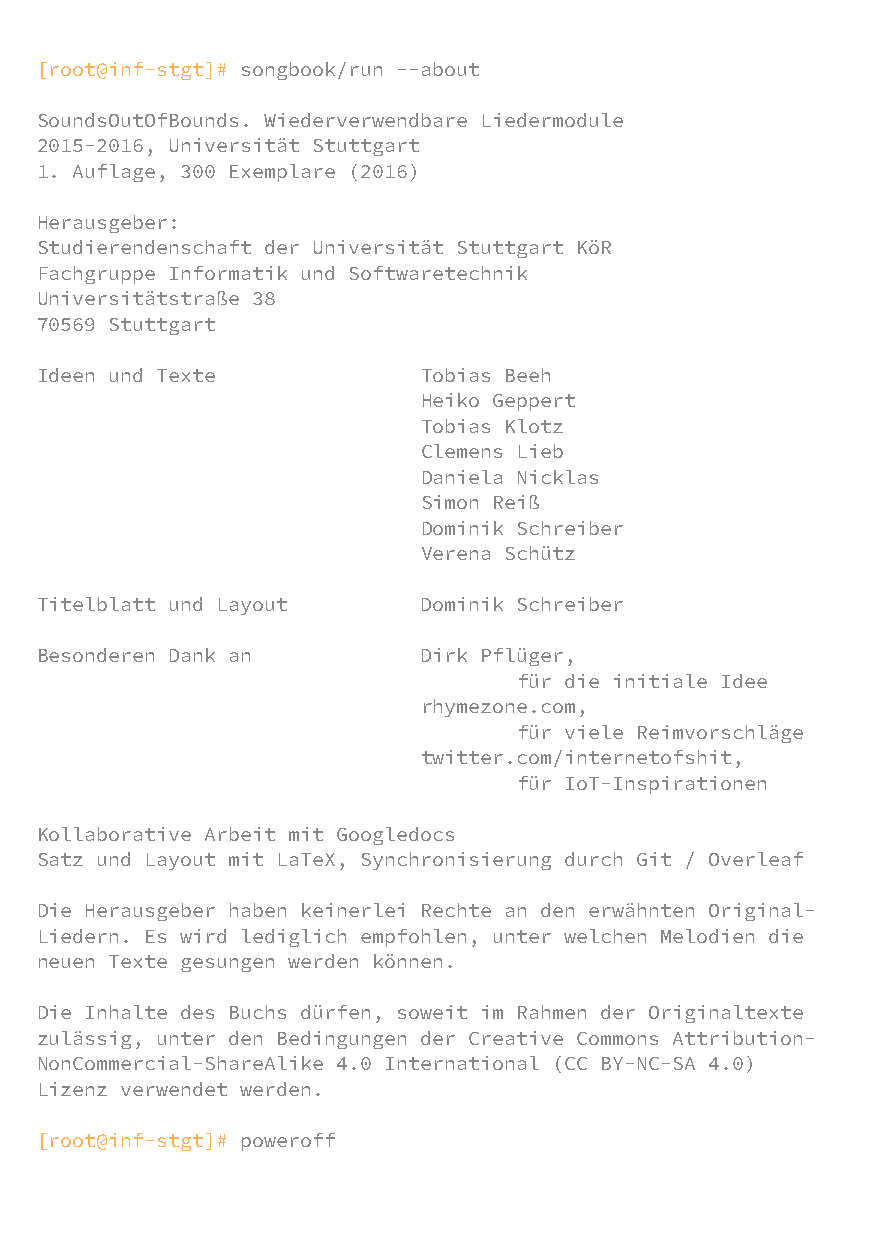
\includegraphics[width=12cm]{hacker-cover-hinten.pdf}\hspace*{\fill}

\thispagestyle{empty}

%\vspace*{3.4cm}

%\section*{Impressum}

%SoundsOutOfBounds. Wiederverwendbare Liedermodule

%Ein Informatik-Liederbuch, herausgegeben von der Fachschaft für Informatik und Softwaretechnik. 2015-2016, Universität Stuttgart \\

%\begin{tabularx}{\columnwidth}{Xr}
%	Titelblatt, Layout &  Dominik Schreiber \\
%	\ \\
%	Ideen und Texte & Tobias Beeh \\
% & Heiko Geppert \\
% & Tobias Klotz \\
% & Clemens Lieb \\
% & Prof. Dr. Daniela Nicklas \\
% & Simon Reiß \\
% & Dominik Schreiber \\
%	\ \\
%	Besonderer Dank an & Junior-Prof. Dirk Pflüger, für die initiale Idee \\
% & rhymezone.com, für viele Reimvorschläge \\
% & twitter.com/internetofshit, für IoT-Inspirationen \\
% & \texttt{127.0.0.1} (Ihr seid die Besten!) \\
%\end{tabularx}

%\ \\

%Kollaborative Arbeit mit Googledocs \\
%Satz und Layout mit \LaTeX , Synchronisierung durch Overleaf \\

%Die Herausgeber haben keinerlei Rechte an den erwähnten Original-Liedern. Es wird lediglich empfohlen, unter welchen Melodien die neuen Texte gesungen werden können. \\

%Die Liedtexte dürfen, soweit im Rahmen der Originaltexte zulässig, weiterverbreitet und non-kommerziell wiederverwendet werden, wenn die Autoren Erwähnung finden.
	
\end{document}